\ifspanish

\question Considere el problema de decisión binario dado por $P_H(1) = 2 P_H(0)$ y verosimilitudes:
$$
\begin{array}{ll} 
	p_{X|H}(x | 0) = 2(1- x),  & 0 \leq x \leq 1  \\
	p_{X|H}(x | 1) = 2 x - 1,  & \dfrac{1}{2} \leq x \leq  \dfrac{3}{2}		  
\end{array}
$$
\begin{parts}
\part Determine el decisor bayesiano para los costes $c_{00} = c_{11} = 0$, $c_{10} = 4 c_{01} > 0$.
\part Determine el decisor de Neyman-Pearson dado por $P_{\rm FA} \le 0.04$.
\part Determine, en función del parámetro $\alpha$, las probabilidades de detección y falsa alarma de la familia de decisores de la forma 
	 $$x \dunodcero \alpha$$
\part Represente gráficamente (de forma aproximada) la curva característica de operación (ROC), tomando $\alpha$ como parámetro libre, e indicando cómo varía el punto de trabajo del decisor en función de su valor.
\part Indique si los decisores de los apartados (a) y (b) se corresponden con algún punto de la ROC y, en su caso, indique con cuál(es).

\end{parts}

\begin{solution}

\begin{parts}
\part El decisor bayesiano para los costes dados esta dado por la regla de decisión:
\begin{align*}
(c_{01} &- c_{11}) P_H(1) p_{X|H}(x|1) \dunodcero (c_{10} - c_{00}) P_H(0) p_{X|H}(x|0) \\
	& \Leftrightarrow \quad c_{01} 2 P_H(0) p_{X|H}(x|1) \dunodcero 4 c_{01} P_H(0) p_{X|H}(x|0) \\
	& \Leftrightarrow \quad p_{X|H}(x|1) \dunodcero 2 p_{X|H}(x|0) \\
	& \Leftrightarrow \quad 
	      \left[\begin{array}{ll}
		        D = 0,                   & \text{if } 0 \le x \le \frac12 \\
		        2 x-1 \dunodcero 4(1-x), & \text{if } \frac12 \le x \le 1 \\
		        D = 1,                   & \text{if } 1 \le x \le \frac32
		        \end{array}
		  \right.   \\
	& \Leftrightarrow \quad 
	      \left[\begin{array}{ll}
		            D = 0,                 & \text{if } 0 \le x \le \frac12 \\
		            x \dunodcero \frac56,  & \text{if } \frac12 \le x \le 1 \\
		            D = 1,                 & \text{if } \frac32 \le x \le 1  
		         \end{array}
		  \right.   \\
	& \Leftrightarrow \quad 
	      x \dunodcero \frac56
\end{align*}
\part El LRT para umbral $\lambda \ge 0$ tiene la forma
\begin{align*}
p_{X|H}(x|1) \dunodcero \lambda p_{X|H}(x|0)
  & \Leftrightarrow \quad 
	  \left[\begin{array}{ll}
            D = 0,                          & \text{if } 0 \le x \le \frac12 \\
		    2x-1 \dunodcero 2\lambda (1-x), & \text{if } \frac12 \le x \le 1 \\
		    D = 1,                          & \text{if } 1 \le x \le \frac32
		    \end{array}
	  \right.   \\
  & \Leftrightarrow \quad 
      \left[\begin{array}{ll}
  	      D = 0,                                        & \text{if } 0 \le x \le \frac12 \\
  	      x \dunodcero \frac{2\lambda+1}{2(1+\lambda)}, & \text{if } \frac12 \le x \le 1 \\
  	      D = 1,                                        & \text{if } 1 \le x \le \frac32
  	      \end{array}
  	  \right.   \\
  & \Leftrightarrow \quad x \dunodcero \alpha
\end{align*}
donde $\alpha = \frac{2 \lambda + 1}{2(1+\lambda)} \in [\frac12, 1]$.

La probabilidad de falsa alarma será
\begin{align*}
P_{\rm FA} &= P_{D|H}(1|0) 
            = P\{x \ge \alpha | H=0\} \\
           &= \int_\alpha^\infty p_{X|H}(x|0) dx 
            = \int_\alpha^1 2(1-x) dx \\
           &= (1-\alpha)^2
\end{align*}
Tomando $P_{\rm FA}\le 0.04$, resulta $(1-\alpha)^2 = 0.04$, luego $\alpha=0.8$ y el decisor NP es
\begin{align*}
x \dunodcero 0.8
\end{align*}

\part De acuerdo con lo visto en el apartado (b), la probabilidad de falsa alarma, para cualquier $\alpha \in [0, \frac32]$ será:
\begin{align*}
P_{\rm FA} 
  &= \left[\begin{array}{ll} 
	       (1-\alpha)^2  & \quad 0 < \alpha < 1         \\
	       0             & \quad 1 < \alpha < \frac32
  	       \end{array}  
  	 \right.  
\end{align*}
Análogamente, la probabilidad de detección será
\begin{align*}
P_{\rm D} 
	&= P_{D|H}(1|1) 
     = P\{x \le \alpha | H=1 \}              
     = \int_\alpha^\infty p_{X|H}(x|1) dx  \\
    &= \left[\begin{array}{ll} 
			 1                              & \quad 0 < \alpha < \frac12 \\	  
			 \int_\alpha^\frac32 (2x-1) dx  & \quad \frac12 < \alpha < \frac32
  			 \end{array}  
	   \right.  	 \\
    &= \left[\begin{array}{ll} 
			 1                                  & \quad 0 < \alpha < \frac12	\\	  
			 1 - \left(\alpha-\frac12\right)^2  & \quad \frac12 < \alpha < \frac32   
  			 \end{array}  
	   \right.  	
\end{align*}

\part Basta con obtener algunos puntos significativos, y dibujar la ROC de forma aproximada. Por ejemplo:
\begin{align*}
\begin{array}{llll} 
  \alpha=0       & \Rightarrow & P_{\rm FA}=1,       & P_{\rm D}= 1 \\
  \alpha=\frac12 & \Rightarrow & P_{\rm FA}=\frac14, & P_{\rm D}= 1 \\
  \alpha=\frac34 & \Rightarrow & P_{\rm FA}=\frac14, & P_{\rm D}= \frac{15}{16} \\
  \alpha=1       & \Rightarrow & P_{\rm FA}=0,       & P_{\rm D}= \frac34 \\
  \alpha=\frac32 & \Rightarrow & P_{\rm FA}=0,       & P_{\rm D}= 0
\end{array}
\end{align*}

\begin{center}
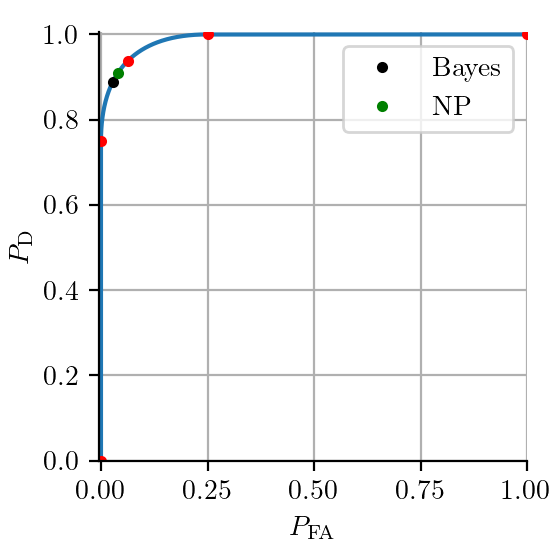
\includegraphics[width=4.5cm]{Figuras/Px06_ROC.png}
\end{center}

\part El decisor bayesiano se corresponde con el caso $\alpha= \frac56$. El decisor NP es el caso $\alpha=0.8$. Sus respectivas posiciones en la ROC se indican en la figura.
\end{parts}
\end{solution}

\else

\question Consider a binary decision problem with $P_H(1) = 2 P_H(0)$ and likelihoods:
$$
\begin{array}{ll} 
	p_{X|H}(x | 0) = 2(1- x),  & 0 \leq x \leq 1  \\
	p_{X|H}(x | 1) = 2 x - 1,  & \dfrac{1}{2} \leq x \leq  \dfrac{3}{2}		  
\end{array}
$$
\begin{parts}
\part Find the Bayesian decision-maker for cost policy $c_{00}=c_{11}=0$, $c_{10}=4c_{01} > 0$.
\part Determine the Neyman-Pearson classifier with $P_{\rm FA} = 0.04$.
\part Obtain, as a function of parameter $\alpha$, the false alarm and detection probabilities for the family of decision-makers with analytic shape
	 $$x \dunodcero \alpha$$
\part Plot (in an approximate manner) the operating characteristic (ROC) curve, taking $\alpha$ as the free parameter, and illustrating how the operation point of the decision-maker changes as a function of the value of such parameter.
\part Indicate whether the decision-makers obtained in (a) and (b) correspond to certain operation points of the previous ROC and, if so, identify it (or them).

\end{parts}

\begin{solution}

\begin{parts}
\part The Bayesian decision-maker for the given costs is given by the decision rule
\begin{align*}
(c_{01} &- c_{11}) P_H(1) p_{X|H}(x|1) \dunodcero (c_{10} - c_{00}) P_H(0) p_{X|H}(x|0) \\
	& \Leftrightarrow \quad c_{01} 2 P_H(0) p_{X|H}(x|1) \dunodcero 4 c_{01} P_H(0) p_{X|H}(x|0) \\
	& \Leftrightarrow \quad p_{X|H}(x|1) \dunodcero 2 p_{X|H}(x|0) \\
	& \Leftrightarrow \quad 
	      \left[\begin{array}{ll}
		        D = 0,                   & \text{if } 0 \le x \le \frac12 \\
		        2 x-1 \dunodcero 4(1-x), & \text{if } \frac12 \le x \le 1 \\
		        D = 1,                   & \text{if } 1 \le x \le \frac32
		        \end{array}
		  \right.   \\
	& \Leftrightarrow \quad 
	      \left[\begin{array}{ll}
		            D = 0,                 & \text{if } 0 \le x \le \frac12 \\
		            x \dunodcero \frac56,  & \text{if } \frac12 \le x \le 1 \\
		            D = 1,                 & \text{if } \frac32 \le x \le 1  
		         \end{array}
		  \right.   \\
	& \Leftrightarrow \quad 
	      x \dunodcero \frac56
\end{align*}
\part The LRT for threshold $\lambda \ge 0$ has the form
\begin{align*}
p_{X|H}(x|1) \dunodcero \lambda p_{X|H}(x|0)
  & \Leftrightarrow \quad 
	  \left[\begin{array}{ll}
            D = 0,                          & \text{if } 0 \le x \le \frac12 \\
		    2x-1 \dunodcero 2\lambda (1-x), & \text{if } \frac12 \le x \le 1 \\
		    D = 1,                          & \text{if } 1 \le x \le \frac32
		    \end{array}
	  \right.   \\
  & \Leftrightarrow \quad 
      \left[\begin{array}{ll}
  	      D = 0,                                        & \text{if } 0 \le x \le \frac12 \\
  	      x \dunodcero \frac{2\lambda+1}{2(1+\lambda)}, & \text{if } \frac12 \le x \le 1 \\
  	      D = 1,                                        & \text{if } 1 \le x \le \frac32
  	      \end{array}
  	  \right.   \\
  & \Leftrightarrow \quad x \dunodcero \alpha
\end{align*}
where $\alpha = \frac{2 \lambda + 1}{2(1+\lambda)} \in [\frac12, 1]$. The false alarm probability is
\begin{align*}
P_{\rm FA} &= P_{D|H}(1|0) 
            = P\{x \ge \alpha | H=0\} \\
           &= \int_\alpha^\infty p_{X|H}(x|0) dx 
            = \int_\alpha^1 2(1-x) dx \\
           &= (1-\alpha)^2
\end{align*}
Taking $P_{\rm FA}\le 0.04$, we get $(1-\alpha)^2 = 0.04$, thus $\alpha=0.8$ and the NP decision-maker is
\begin{align*}
x \dunodcero 0.8
\end{align*}

\part According to part (b), the false alarm probability, for any $\alpha \in [0, \frac32]$ is
\begin{align*}
P_{\rm FA} 
  &= \left[\begin{array}{ll} 
	       (1-\alpha)^2  & \quad 0 < \alpha < 1         \\
	       0             & \quad 1 < \alpha < \frac32
  	       \end{array}  
  	 \right.  
\end{align*}
In a similar way, the detection probability is
\begin{align*}
P_{\rm D} 
	&= P_{D|H}(1|1) 
     = P\{x \le \alpha | H=1 \}              
     = \int_\alpha^\infty p_{X|H}(x|1) dx  \\
    &= \left[\begin{array}{ll} 
			 1                              & \quad 0 < \alpha < \frac12 \\	  
			 \int_\alpha^\frac32 (2x-1) dx  & \quad \frac12 < \alpha < \frac32
  			 \end{array}  
	   \right.  	 \\
    &= \left[\begin{array}{ll} 
			 1                                  & \quad 0 < \alpha < \frac12	\\	  
			 1 - \left(\alpha-\frac12\right)^2  & \quad \frac12 < \alpha < \frac32   
  			 \end{array}  
	   \right.  	
\end{align*}

\part Obtaining some sample points and plotting the ROC in an approximate manner will suffice. For instance:
\begin{align*}
\begin{array}{llll} 
  \alpha=0       & \Rightarrow & P_{\rm FA}=1,       & P_{\rm D}= 1 \\
  \alpha=\frac12 & \Rightarrow & P_{\rm FA}=\frac14, & P_{\rm D}= 1 \\
  \alpha=\frac34 & \Rightarrow & P_{\rm FA}=\frac14, & P_{\rm D}= \frac{15}{16} \\
  \alpha=1       & \Rightarrow & P_{\rm FA}=0,       & P_{\rm D}= \frac34 \\
  \alpha=\frac32 & \Rightarrow & P_{\rm FA}=0,       & P_{\rm D}= 0
\end{array}
\end{align*}

\begin{center}
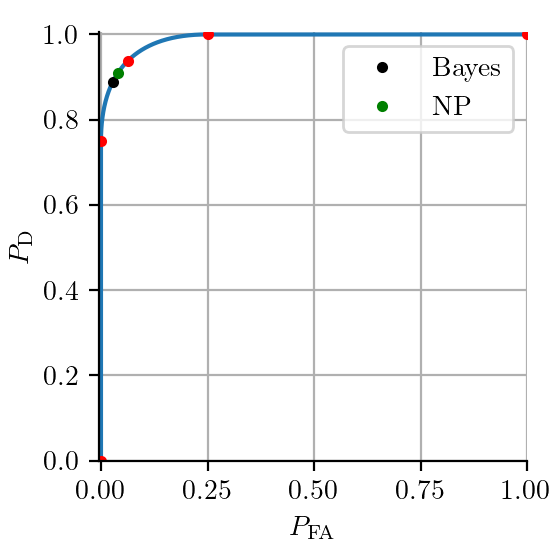
\includegraphics[width=4.5cm]{Figuras/Px06_ROC.png}
\end{center}

\part The Bayesian decision maker is equivalent $\alpha= \frac56$. The NP decision-maker is equivalent to $\alpha=0.8$. Their respective locations in the ROC are shown in the figure.
\end{parts}
\end{solution}

\fi